\section{Discrete Random Variables}

\subsection{Random Variables and Probability Density Function}

\begin{frame}{Random Variables and Probability Density Function}

\justifying
\structb{Definition.} Let $S$ be a sample space and $\Omega$ a \underline{countable} subset of $\R$. A \highlightg{discrete random variable} is a map
\begin{align*}
X: S\rightarrow \Omega
\end{align*}
together with a function
\begin{align*}
f_X: \Omega \rightarrow \R
\end{align*}
having the properties that
\begin{itemize}
	\item[(i)] $f_X(x) \geq 0$ for all $x\in \Omega$ and
	\item[(ii)] $\displaystyle \sum_{x\in \Omega} f_X(x) = 1$.
\end{itemize}
The function $f_X$ is called the \highlightg{probability density function} or \highlightg{probability distribution} of $X$. A random variable is given by the pair $(X, f_X)$.

\end{frame}


\subsection{Cumulative Distribution Function}

\begin{frame}{Cumulative Distribution Function}

\justifying
\structb{Definition.} The \highlightg{cumulative distribution function} of a random variable is defined as
\begin{align*}
F_X: \R\rightarrow \R, \qquad F_X(x) := P[X\leq x].
\end{align*}
For a discrete random variable,
\begin{align*}
F_X(x) = \sum_{y\leq x} f_X(y).
\end{align*}

\end{frame}

\subsection{Expectation and Variance}

\begin{frame}{Expectation and Variance}

\structb{Definition.} Let $(X, f_X)$ be a discrete random variable.
\begin{itemize}
	\justifying
	\item The \highlightg{expected value} or \highlightg{expectation} of $X$ is 
	\begin{align*}
	\mu_X = \U{E}[X] := \sum_{x\in \Omega} x\cdot f_X(x),
	\end{align*}
	provided that the sum (possibly series, if $\Omega$ is infinite) on the right converges absolutely.
	\item The \highlightg{variance} is defined by
	\begin{align*}
	\sigma_X^2 = \U{Var}[X] := \U{E}\left[(X - \U{E}[X])^2 \right]
	\end{align*}
	which is defined as long as the right-hand side exists.
	\item The \highlightg{standard deviation} is $\sigma_X = \sqrt{\U{Var}[X]}$.
\end{itemize}

\end{frame}

\begin{frame}{Properties}

\begin{itemize}
	\justifying
	\item \underline{Expectation}.
	\justifying
	\begin{enumerate}[(a).]
		\justifying
		\item Suppose $\varphi: \Omega \rightarrow \R$ is some function, then
		\begin{align*}
		\U{E}[\varphi\circ X] = \displaystyle \sum_{x\in \Omega} \varphi(x) \cdot f_X(x).
		\end{align*}
		\item $\U{E}[aX + bY + c] = a\U{E}[X] + b\U{E}[Y] + c$, where $a, b, c\in \R$ and $X, Y$ are random variables.
		\item $\displaystyle\U{E}\left[\sum_{i=1}^n X_i \right]  = \sum_{i=1}^n \U{E}[X_i]$, if each expectation exists.
		\item If $X_1, \ldots, X_n$ are independent random variables with finite expectations, and $g_i, i = 1, \ldots, n$ are functions, then 
		\begin{align*}
		\U{E}\left[\prod_{i=1}^n X_i \right] = \prod_{i=1}^n \U{E}[X_i], \quad \U{E}\left[\prod_{i=1}^n g_i(X_i) \right] = \prod_{i=1}^n \U{E}[g_i(X_i)].
		\end{align*}
	\end{enumerate}
\end{itemize}


\end{frame}

\begin{frame}{Properties}

\begin{itemize}
	\justifying
	\item \underline{Variance}.
	\begin{enumerate}[(a).]
		\justifying
		\item $\U{Var}[X] = \U{E}[X^2] - \U{E}[X]^2$.
		\item $\U{Var}[aX + b] = a^2\U{Var}[X]$, where $a, b \in \R$.
		\item If $X_1, \ldots, X_n$ are independent random variables, then 
		\begin{align*}
		\U{Var}\left[\sum_{i=1}^n a_iX_i \right]  = \sum_{i=1}^n a_i^2\U{Var}[X_i].
		\end{align*}
	\end{enumerate}
	\highlightr{Note.} If $X$ and $Y$ are not independent, then according to definitions,
	\begin{align*}
	\U{Var}[X + Y] & = \U{E}\left[\left(X + Y - (\mu_X + \mu_Y) \right)^2 \right] \\
	& = \U{E}\left[(X-\mu_X)^2 \right] + \U{E}\left[(Y - \mu_Y)^2 \right] + \\
	& \qquad \qquad \qquad + 2\U{E}\left[(X-\mu_X)(Y-\mu_Y) \right] \\
	& \neq \U{Var}[X] + \U{Var}[Y].
	\end{align*}
\end{itemize}


\end{frame}


\subsection{Moment-Generating Function}

\begin{frame}{Ordinary and Central Moments}

\justifying
\structb{Definition.} The \highlightg{$n^{th}$ (ordinary) moments} of a random variable $X$ is given by
\begin{align*}
\U{E}[X^n], \qquad n\in \N.
\end{align*}
The \highlightg{$n^{th}$ central moments} of $X$ is given by
\begin{align*}
\U{E}\left[\left(\frac{X-\mu}{\sigma} \right)^n \right], \qquad \U{where\ } n = 3, 4, 5, \ldots
\end{align*}

\end{frame}

\begin{frame}{Moment-Generating Function}

\justifying
\structb{Definition.} Let $(X, f_X)$ be a random variable and such that the sequence of moments $\U{E}[X^n], n\in \N$, exists. If the power series 
\begin{align*}
m_X(t) := \sum_{k=0}^{\infty} \frac{\U{E}[X^k]}{k!} t^k
\end{align*}
has radius of convergence $\varepsilon > 0$, the thereby defined function
\begin{align*}
m_X(t): (-\varepsilon, \varepsilon) \rightarrow \R
\end{align*}
is called the \highlightg{moment-generating function} for $X$.

\end{frame}


\begin{frame}{Moment-Generating Function}

\justifying
\structb{Theorem.} Let $\varepsilon > 0$ be given such that $\U{E}[e^{tX}]$ exists and has a power series expansion in $t$ that converges for $|t| < \varepsilon$. Then the moment-generating function exists and 
\begin{align*}
m_X(t) = \U{E}[e^{tX}] \qquad \U{for\ } |t| < \varepsilon.
\end{align*}
Furthermore, 
\begin{align*}
E[X^k] = \frac{\U{d}^k m_X(t)}{\U{d}t^k}\bigg|_{t=0}.
\end{align*}
We can hence calculate the moments of $X$ by differentiating the moment-generating function.

\end{frame}

\begin{frame}{Moment-Generating Function}

\structb{Properties.} 
\begin{itemize}
	\justifying
	\item $X$ is a random variable and $Y = aX + b, a, b\in \R$, then for every $t$ such that $m_X(at)$ is finite,
	\begin{align*}
	m_Y(t) = e^{bt} m_X(at).
	\end{align*}
	\item Suppose $X_1, \ldots, X_n$ are $n$ independent random variables, then for every value that $m_{X_i}(t)$ is finite for all $i = 1, \ldots, n$,
	\begin{align*}
	m_X(t) = \prod_{i=1}^n m_{X_i}(t), \qquad X = X_1 + \cdots + X_n.
	\end{align*}
\end{itemize}

\end{frame}


\begin{frame}{Moment-Generating Function}

\justifying
\structb{Example 1.} Suppose that $X$ is a random variable with the moment-generating function 
\begin{align*}
m_X: \R\rightarrow \R, \qquad m_X(t) = e^{t^2 + 3t}.
\end{align*}
Find the mean and variance of $X$.\\
~\\
\uncover<2>{
	\structb{Solution.} We calculate
	\begin{align*}
	m_X'(t) = (2t+3) e^{t^2 + 3t}, \quad m_X''(t) = (2t+3)^2e^{t^2+3t} + 2e^{t^2+3t}.
	\end{align*}
	Therefore,
	\begin{align*}
	\mu = m_X'(0) = 3, \quad \sigma^2 = \U{E}[X^2] - \U{E}[X]^2 = m_X''(0) - \mu^2 = 2.
	\end{align*}
}

\end{frame}


\section{Common Distributions of Discrete Random Variables}

\subsection{Binomial Distribution}

\begin{frame}{Bernoulli Distribution}

\justifying
\structb{Definition.} A random variable $(X, f_X)$ has a \highlightg{Bernoulli distribution} with parameter $p, 0 < p < 1$ if the probability density function is defined by
\begin{align*}
f_X: \{0, 1\} \rightarrow \R, \qquad f_X(x) = \left\{
\begin{array}{ll}
1-p, & \U{if\ } x = 0, \\
p, & \U{if\ } x = 1.
\end{array}
\right.
\end{align*}
\structb{Interpretation.} Describe the probability of success $f_X(1)$ or failure $f_X(0)$ of a trial, given the probability of success is $p$.

\end{frame}

\begin{frame}{Bernoulli Distribution}

\justifying
\structb{Mean, variance, and M.G.F.}
\begin{itemize}
	\justifying
	\item \underline{Mean}.
	\begin{align*}
	\U{E}[X] = 0\cdot (1-p) + 1\cdot p = p.
	\end{align*}
	\item \underline{Variance}.
	\begin{align*}
	\U{Var}[X] = \U{E}[X^2] - \U{E}[X]^2 = p - p^2 = p(1-p).
	\end{align*}
	\item \underline{M.G.F.}
	\begin{align*}
	m_X: \R\rightarrow \R, \qquad m_X(t) = (1-p) + e^tp.
	\end{align*}
\end{itemize}

\end{frame}

\begin{frame}{Binomial Distribution}

\justifying
\structb{Definition.} A random variable $(X, f_X)$ has a \highlightg{binomial distribution} with parameter $n\in \N\setminus\{0\}$ and $p, 0 < p < 1$ if it has probability density function
\begin{align*}
f_X: \{0, \ldots, n\} \rightarrow \R, \qquad f_X(x) = \binom{n}{x} p^x(1-p)^{n-x}.
\end{align*}
~\\
\structb{Interpretation.} $f_X(x)$ is the probability of obtaining $x$ successes in $n$ independent and identical Bernoulli trials with parameter $p$.


\end{frame}


\begin{frame}{Binomial Distribution}

\justifying
\structb{Mean, variance and M.G.F.} 
\begin{itemize}
	\justifying
	\item \underline{Mean}.
	\begin{align*}
	\U{E}[X] & = \sum_{i=1}^n \U{E}[X_i] = np.
	\end{align*}
	\item \underline{Variance}. 
	\begin{align*}
	\U{Var}[X] = \sum_{i=1}^n\U{Var}[X_i] = np(1-p).
	\end{align*}
	\item \underline{M.G.F.}
	\begin{align*}
	m_X: \R\rightarrow\R, \qquad m_X(t) = \U{E}[e^{tX}] = \prod_{i=1}^n\U{E}[e^{tX_i}] = (1 - p + pe^t)^n.
	\end{align*}
\end{itemize}

\end{frame}

\subsection{Geometric Distribution}

\begin{frame}{Geometric Distribution}

\justifying
\structb{Definition.} A random variable $(X, f_X)$ has \highlightg{geometric distribution} with parameter $p, 0 < p < 1$ if the probability density function is given by
\begin{align*}
f_X: \N\setminus \{0\} \rightarrow \R, \qquad f_X(x) = (1-p)^{x-1} p.
\end{align*}
~\\
\structb{Interpretation.} $f_X(x)$ is the probability of $x$ failures before the first success in the Bernoulli trials, given the probability of success for each trial is $p$.

\end{frame}

\begin{frame}{Geometric Distribution}

\justifying
\structb{Mean, variance and M.G.F.} 
\begin{itemize}
	\justifying
	\item \underline{Mean}.
	\begin{align*}
	\U{E}[X] = \frac{1}{p}.
	\end{align*}
	\item \underline{Variance}.
	\begin{align*}
	\U{Var}[X] = \frac{1-p}{p^2}.
	\end{align*}
	\item \underline{M.G.F.}
	\begin{align*}
	m_X: (-\infty, -\ln(1-p)) \rightarrow\R, \qquad m_X(t) = \frac{pe^t}{1-(1-p)e^t}.
	\end{align*}
\end{itemize}

\end{frame}

\subsection{Pascal, Negative Binomial Distribution}

\begin{frame}{Pascal Distribution}

\justifying
\structb{Definition.} A random variable $(X, f_X)$ has the \highlightg{Pascal distribution} with parameters $p, 0 < p < 1$ and $r\in \N\setminus\{0\}$ if the probability density function is given by
\begin{align*}
f_X:\{r, r + 1, \ldots\} \rightarrow \R, \qquad  f_X(x) = \binom{x-1}{r-1} p^r(1-p)^{x-r}.
\end{align*}
~\\
\structb{Interpretation.} $f_X(x)$ is the probability of obtaining the $r$-th success in the $x$-th Bernoulli trail, given the probability of success for each trail is $p$.

\end{frame}

\begin{frame}{Pascal Distribution}

\justifying
\structb{Mean, variance and M.G.F.} 
\begin{itemize}
\justifying
\item \underline{Mean}.
\begin{align*}
\U{E}[X] = \frac{r}{p}.
\end{align*}
\item \underline{Variance}. Let $q = 1 - p$,
\begin{align*}
\U{Var}[X] = \frac{rq}{p^2}.
\end{align*}
\item \underline{M.G.F.}
\begin{align*}
m_X: (-\infty, -\ln q) \rightarrow \R, \qquad m_X(t) = \frac{(pe^t)^r}{(1-qe^t)^r}.
\end{align*}
\end{itemize}

\end{frame}


\begin{frame}{Negative Binomial Distribution}

\justifying
\structb{Definition.} A random variable $(X, f_X)$ has the \highlightg{negative binomial distribution} with parameters $r$ and $p$ if the probability density function is given by
\begin{align*}
f_X: \N \rightarrow \R, \qquad f_X(x) = \binom{x+r-1}{r-1} p^r(1-p)^{x}.
\end{align*}
~\\
\structb{Interpretation.} $f_X(x)$ is the probability of $x$ failures before first obtaining $r$ successes in Bernoulli trials, given the probability for each success is $p$.

\end{frame}

\begin{frame}{Negative Binomial Distribution}

\justifying
\structb{Mean, variance and M.G.F.} 
\begin{itemize}
\justifying
\item \underline{Mean}. Let $q = 1 - p$,
\begin{align*}
\U{E}[X] = \frac{rp}{q}.
\end{align*}
\item \underline{Variance}.
\begin{align*}
\U{Var}[X] = \frac{rp}{q^2}.
\end{align*}
\item \underline{M.G.F.}
\begin{align*}
m_X: (-\infty, -\ln q) \rightarrow \R, \qquad m_X(t) = \frac{p^r}{(1-qe^t)^r}.
\end{align*}
\end{itemize}

\end{frame}

\subsection{Poisson Distribution}

\begin{frame}{Poisson Distribution}

\justifying
\structb{Definition.} A random variable $X$ has the \highlightg{Poisson distribution} with parameter $k > 0$ if probability density function is given by
\begin{align*}
f_X: \N \rightarrow \R, \qquad f_X(x) = \frac{k^xe^{-k}}{x!}
\end{align*}
~\\
\structb{Interpretation.} $f_X(x)$ is the probability of $x$ arrivals in the time interval $[0, t]$ with arrival rate $\lambda > 0$, and $k = \lambda t$. \\
~\\
~~~~\emph{``...which describes the occurrence of events that occur at a \underline{constant rate} and \underline{continuous environment}.''} \\

\end{frame}

\begin{frame}{Poisson Distribution}

\structb{Interpretation.} \emph{Constant rate} and \emph{continuous environment}?
\begin{itemize}
	\justifying
	\item \underline{Continuous environment}. Not limited to time intervals, but also subregions of two- or three-dimensional regions or sublengths of a linear distance, and any regions that can be divided into arbitrarily small pieces.
	\item \underline{Constant rate}. The probability of an occurrence during each very short interval (region) must be approximately proportional to the length (area, volume) of that interval (region).
\end{itemize}
\uncover<2>{
\structb{Examples.} Poisson process can be used to model
\begin{enumerate}[(a).]
	\justifying
	\item the number of particles that strike a certain target at a constant rate in a particular period;
	\item the number of oocysts that occur in a water supply system given constant rate of occurrence per liter;
\end{enumerate}
and many more.
}

\end{frame}

\begin{frame}{Poisson Distribution}

\justifying
\structb{Mean, variance and M.G.F.} 
\begin{itemize}
\justifying
\item \underline{Mean}.
\begin{align*}
\U{E}[X] = k.
\end{align*}
\item \underline{Variance}.
\begin{align*}
\U{Var}[X] = k.
\end{align*}
\item \underline{M.G.F.}
\begin{align*}
m_X: \R \rightarrow \R, \qquad m_X(t) = e^{k(e^t-1)}.
\end{align*}
\end{itemize}

\end{frame}

\subsection{Connection of Distributions}

\begin{frame}{Distributions Based on Bernoulli Trials}

\begin{figure}[htbp]
	\centering
	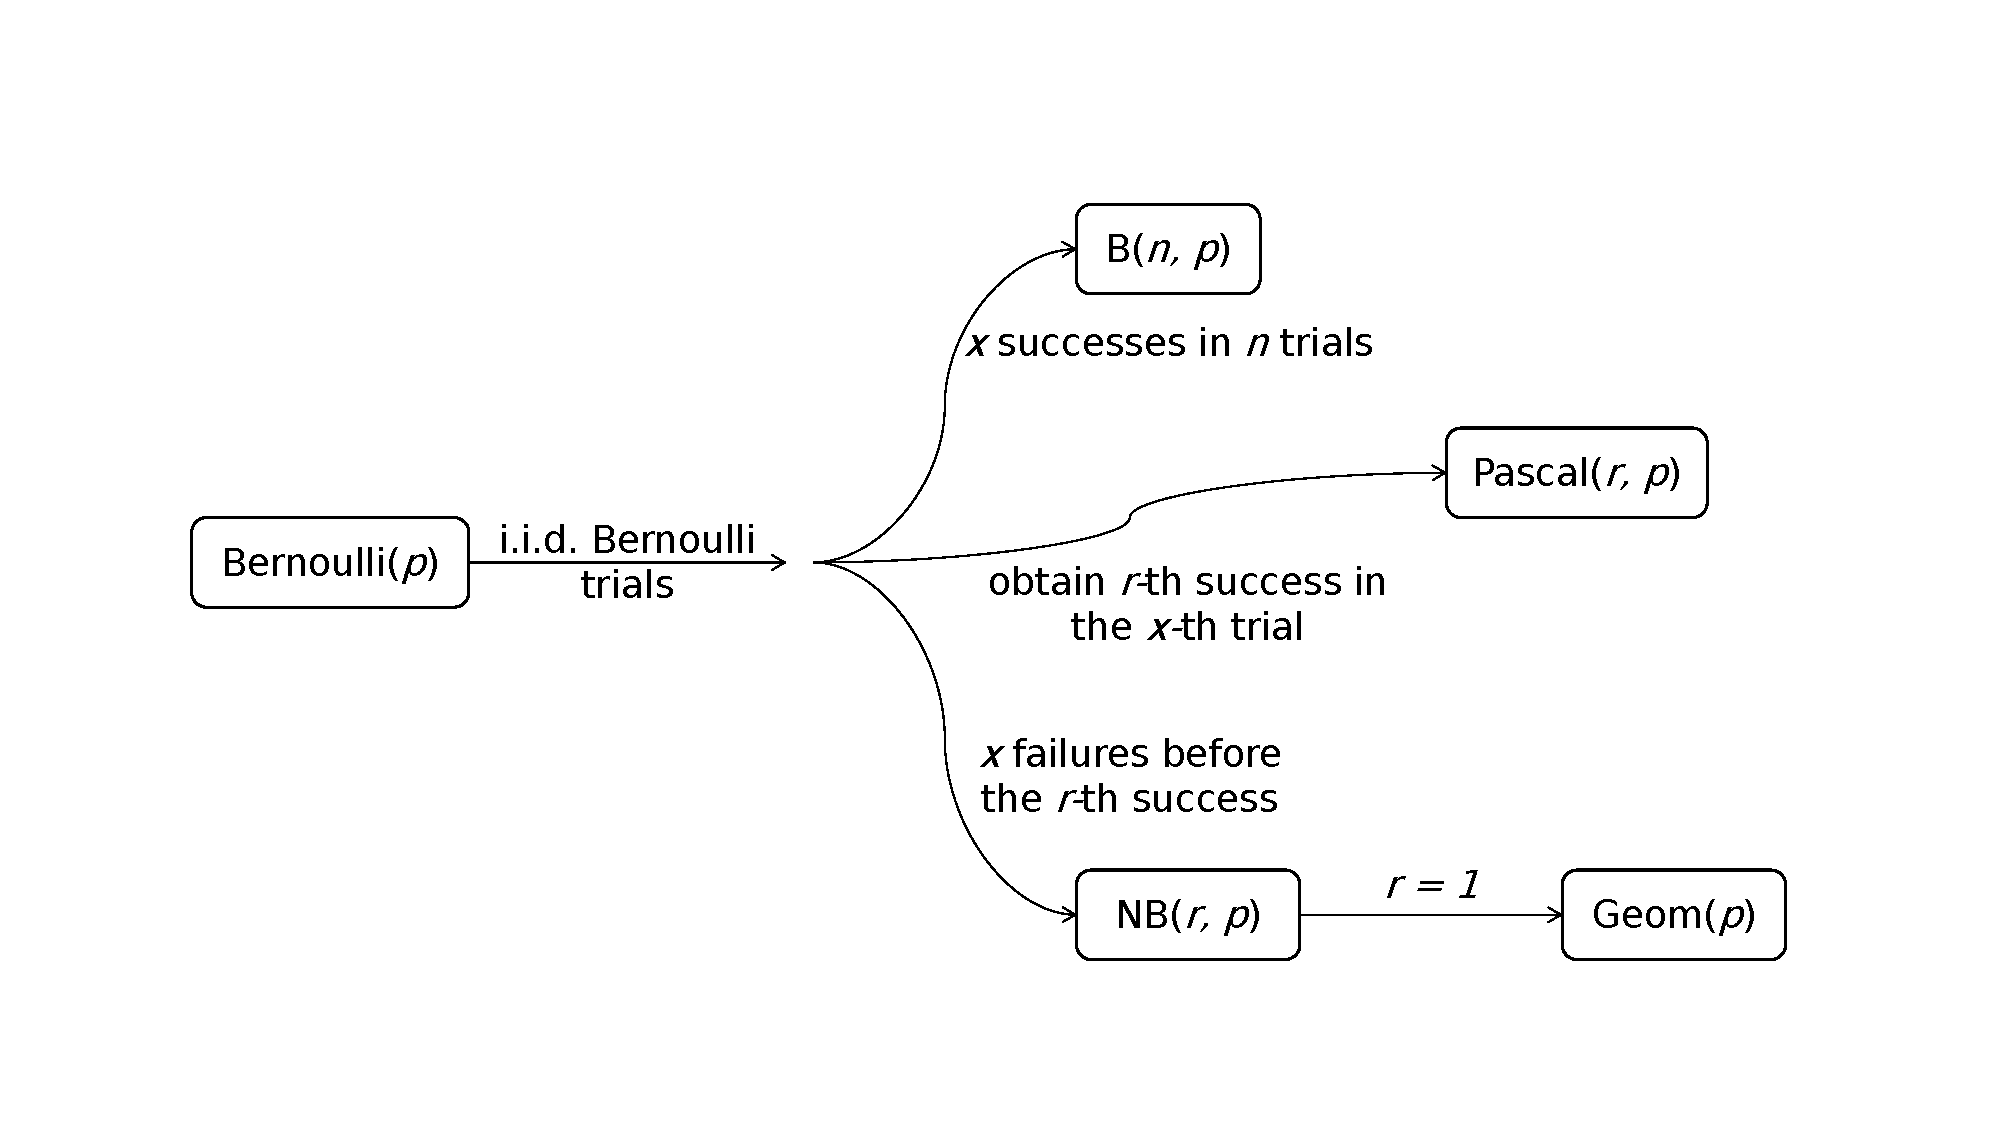
\includegraphics[width=\linewidth]{./images/rc2fig1.pdf}
	\caption{Connections of distributions based on Bernoulli trials.}
\end{figure}

\end{frame}


\begin{frame}{Connections of Distributions}

\begin{itemize}
	\justifying
	\item \underline{Bernoulli $\rightarrow$ Binomial}. $X_1, \ldots, X_n$ are independent random variables,
	\begin{align*}
	X_i\sim \U{Bernoulli}(p) \quad \Rightarrow \quad X = X_1 + \cdots + X_n \sim \U{B}(n, p).
	\end{align*}
	\item \underline{Binomial $\rightarrow$ Binomial}. $X_1, \ldots, X_k$ are independent random variables,
	\begin{align*}
	X_i\sim \U{B}(n_i, p) \quad \Rightarrow\quad X = X_1 + \cdots + X_k \sim \U{B}(n, p),
	\end{align*}
	where $n = n_1 + \cdots + n_k$.
	\item \underline{Geometric $\rightarrow$ Negative binomial}. $X_1, \ldots, X_r$ are independent random variables,
	\begin{align*}
	X_i\sim \U{Geom}(p) \quad \Rightarrow \quad X = X_1 + \cdots + X_r \sim \U{NB}(r, p).
	\end{align*}
\end{itemize}

\end{frame}


\begin{frame}{Connections of Distributions}

\begin{itemize}
	\justifying
	\item \underline{Negative binomial $\rightarrow$ Negative binomial}. $X_1, \ldots, X_n$ are independent random variables,
	\begin{align*}
	X_i\sim \U{NB}(r_i, p) \quad \Rightarrow \quad X = X_1 + \cdots + X_n \sim \U{NB}(r, p),
	\end{align*}
	where $r = r_1 + \cdots + r_n$.
	\item \underline{Poisson $\rightarrow$ Poisson}. $X_1, \ldots, X_n$ are independent random variables,
	\begin{align*}
	X_i\sim \U{Poisson}(k_i) \quad \Rightarrow \quad X = X_1 + \cdots + X_n \sim \U{Poisson}(k),
	\end{align*}
	where $k = k_1 + \cdots + k_n$.
\end{itemize}

\end{frame}


\begin{frame}{Closeness of Binomial Distribution and Poisson Distribution}

\justifying
\structb{Theorem.} For $n\in \N\setminus\{0\}, 0 < p < 1$, suppose $f(x; n, p)$ denotes the probability density function of binomial distribution with parameters $n$ and $p$, while $f(x; k)$ denotes the probability density function of Poisson distribution with parameter $k$. Let $\{p_n\}_{n=1}^{\infty}$ be a sequence of numbers between 0 and 1 such that
\begin{align*}
\lim_{n\rightarrow\infty} np_n = k,
\end{align*}
then
\begin{align*}
\lim_{n\rightarrow \infty} f(x; n, p_n) = f(x; k), \qquad \U{for\ all\ } x = 0, 1, \ldots
\end{align*}
This means we can approximate the binomial distribution with Poisson distribution when $n$ is large. A proof can be found in \texttt{s1.pdf}.

\end{frame}


\section{Exercises}

\subsection{Discrete Random Variables}

\begin{frame}{Exercises}

\justifying
\structb{Exercise 1.} Suppose Keven plays a game where he has probability $p$ to win in each play. When he wins, his fortune is doubled, and when he loses, his fortune is cut in half. If he begins playing with a given fortune $c > 0$, what is the expected value of his fortune after $n$ independent plays?

\end{frame}

\subsection{Common Discrete Distributions}


\begin{frame}{Exercises}

\justifying
\structb{Exercise 2.} For $0 < p < 1$ and $n = 2, 3, \ldots$, determine the value of
\begin{align*}
\sum_{x=2}^n x(x-1)\binom{n}{x} p^x(1-p)^{n-x}.
\end{align*}

\end{frame}


\begin{frame}{Exercises}

\justifying
\structb{Exercise 3.} Suppose that a book with $n$ pages contains on the average $\lambda$ misprints per page. What is the probability that there will be at least $m$ pages which contain more than $k$ misprints?

\end{frame}
